\chapter{Herangehensweise}

\cite[10]{mcg2012} beschreibt \enquote{the experimental process} im Kontext der experimentellen Algorithmusanalyse wie folgt:
\begin{enumerate}
    \item Plane das Experiment:
    \begin{enumerate}[label={(\alph*)}]
        \item Formuliere eine Frage.\label{itm:experiment-formulate-question}
        \item Stelle eine Testumgebung bereit. Die Testumgebung umfasst beispielsweise das Testprogramm, Generatoren der Eingabemengen und Messwerkzeuge.
        \item Gestalte ein Experiment welches die Frage aus \ref{itm:experiment-formulate-question} anspricht. Hier ist beispielsweise festzulegen, welche Eigenschaften gemessen werden, welche Arten von Eingabemengen verwendet werden und mit welchen Eingabegrößen gemessen wird.
    \end{enumerate}
    
    \item Führe das Experiment aus:
    \begin{enumerate}[label={\alph*}]
        \item Führe das Testprogramm aus und sammle die Daten.
        \item Mache durch Datenanalyse relevante Informationen ausfindig. Wurde die Frage nicht beantwortet, gehe zu Schritt 1.
    \end{enumerate}
\end{enumerate}

Um eine Funktion der  praktische Effizienz eines Algorithmus zu ermitteln, gilt es die Laufzeit mit verschiedenen Eingabegrössen zu messen, um sie als Funktion beschreiben zu können. Das Fundament hierfür ist in \prettyref{sec:laufzeiterm} gegeben, eine konkrete Methode zur Ermittlung der praktischen Effizienz wird in \prettyref{sec:funkterm} dargelegt.

Die Beschaffenheit der Eingabemenge --- im Falle von Sortieralgorithmen beispielsweise der Grad der Sortiertheit --- hat oftmals großen Einfluss auf die Effizenz (siehe \prettyref{cha:ergebnisse} und \ldots\nocit). In \prettyref{sec:eingabengen} werden einige Eingabemengen beschrieben.

\section{Laufzeitermittlung}
\label{sec:laufzeiterm}

Ein Algorithmus wird ausgeführt, die Zeit unmittelbar vor (\id{start}) und nach (\id{end}) der Ausführung wird gemessen. Die Laufzeit des Algorithmus ist nun gleich $\id{end} - \id{start}$.

Eine konkrete Implementation einer Klasse zur Messung der Laufzeit eines Algorithmus ist in \prettyref{lst:experiment} gegeben. \ifndef{vwarelease}{\emph{Referenzen zu empirischen Analysen die einen ähnlichen Mechanismus zur Laufzeitermittlung verwenden (kann nicht so schwer sein, was sollen sie sonst verwenden) sind beizufügen.}}{}

\begin{lstlisting}[caption={Implementation einer Klasse zur Ermittlung der Laufzeit eines Algorithmus.}, label=lst:experiment]
class experiment {
	std::function<void()> algorithm;

public:
	using time_t = double;

	|\label{ln:exp-constructor}|explicit experiment(std::function<void()> algorithm)
		: algorithm(std::move(algorithm)) { };

	auto run() const {
		const auto |\id{start}| = std::chrono::steady_clock::now();

		algorithm();

		const auto |\id{end}| = std::chrono::steady_clock::now();

		return std::chrono::duration<time_t, std::micro>{ |\id{end}| - |\id{start}| };
	}
};
\end{lstlisting}

Die Laufzeit eines einfachen Algorithmus kann mit ihrer Hilfe durch
\begin{lstlisting}[numbers=none]
void a1() { ... }
const auto time = experiment(a1).run();
\end{lstlisting}
ermittelt werden, wobei die Zeitspanne in Mikrosekunden ($1\mu s = 10^{-6} s$) angegeben ist.

\paragraph{Algorithmen mit Eingabewerten} Die im Folgenden behandelten Algorithmen haben üblicherweise einen oder mehrere Eingabewerte, sie erfüllen also nicht die Form wie sie vom Konstruktor in \prettyref{lst:experiment}, \prettyref{ln:exp-constructor} erwartet wird.

\begin{lstlisting}[numbers=none]
void |\id{func}|(size_t s) { ... }
const auto |\id{wrapper}| = std::bind(func, 1337);
const auto time = experiment(wrapper).run();
\end{lstlisting}
Im obenstehenden Beispielcode ist \id{func} eine beliebige Funktion die einen Eingabewert hat. \id{wrapper} ist eine Funktion der Form \lstinline{void()} (die also dem Konstruktor aus \prettyref{ln:exp-constructor} übergeben werden kann), welche die Funktion \id{func} mit dem bei ihrer Erstellung übergebenen Wert 1337 aufruft, wenn sie aufgerufen wird.

\section{Eingabengenerierung}
\label{sec:eingabengen}

\ifndef{vwarelease}{\emph{Referenzen anderer Analysen mit gleichen oder überlappenden Eingabearten sind beizufügen.}}{}

Folgende Eingabemengen werden für die Ermittlung der praktischen Effizienz verwendet:

\begin{enumerate}
    \item sortiert
    \item invertiert
    \item zufällig geordnet
\end{enumerate}

Siehe \prettyref{lst:sets} für eine beispielhafte Implementation der obigen Eingabemengearten.

Eine ausführlichere Auswahl an Eingangsmengen welche an einen sie bearbeitenden Algorithmen angepasst ist --- wie sie für eine eingehende Analyse eines einzelnen Algorithmus angebracht wäre --- würde das allgemeiner gesetzte Ziel dieser Arbeit verfehlen.

\section{Funktionsermittlung}
\label{sec:funkterm}

Im gegebenen Kontext ist es das Ziel der \enquote{Funktionsermittlung} eine Funktion in Abhängigkeit der Eingabegröße aufzustellen, welche die Laufzeit darstellt. Die $x$-Werte dieser Funktion stellen also die Größe der Eingabemenge, und die $y$-Werte die Zeit die der Algorithmus bei Eingabe einer Menge dieser Größe benötigt hat, dar (siehe \prettyref{fig:function-determination-example}).

\begin{figure}[ht]
    \centering
    \begin{subfigure}[t]{0.49\linewidth}
        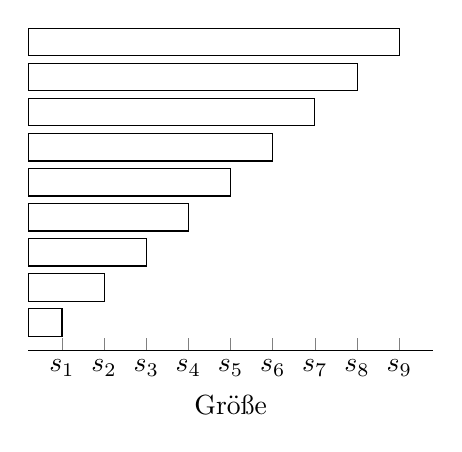
\begin{tikzpicture}
        \begin{axis}[
            xbar,
            xlabel={Größe},
            yticklabels=\empty,
            xtick={1, ..., 9},
            xticklabels={$s_1$, $s_2$, $s_3$, $s_4$, $s_5$, $s_6$, $s_7$, $s_8$, $s_9$},
            scale=0.75,
            axis y line=none,
            axis x line*=bottom,
        ]
            \addplot+ [fill=white, draw=black] coordinates  {(9, 9) (8, 8) (7, 7) (6, 6) (5, 5) (4, 4) (3, 3) (2, 2) (1, 1)};
        \end{axis}
        \end{tikzpicture}
        
        \subcaption{Größe der Eingangsmengen, dargestellt als Balkendiagramm.}
    \end{subfigure}
    \begin{subfigure}[t]{0.49\linewidth}
        \begin{tikzpicture}
        \begin{axis}[
            xlabel={Größe},
            ylabel={Zeit},
            yticklabels=\empty,
            xtick={0, ..., 8},
            xticklabels={$s_1$, $s_2$, $s_3$, $s_4$, $s_5$, $s_6$, $s_7$, $s_8$, $s_9$},
            scale=0.75,
            smooth,
            grid=major,
        ]
            \addplot [] table {data/example};
        \end{axis}
        \end{tikzpicture}

        \subcaption{$f(s)$}
    \end{subfigure}
    \caption{Beispielhafter Funktionsgraph der praktischen Effizienz eines hypothetischen Algorithmus mit Illustration der Eingabemengengrößen.}
    \label{fig:function-determination-example}
\end{figure}

Diese Funktion der praktischen Effizienz kann mithile der Funktion \linebreak[4]\lstinline{benchmark::run} in \prettyref{lst:benchmark} ermittelt werden.

\begin{lstlisting}[label=lst:benchmark, caption={Implementation einer Funktion zur Ermittlung der praktischen Effizienz eines Algorotihmus mit einer bestimmenten Eingabemenge.}]
namespace benchmark {
	using timings_t = std::map<size_t, experiment::time_t>;

	template<class A, class S>
	timings_t run(A algorithm, S set, int total_chunks) {
		timings_t timings;

		const size_t set_size = set.size();

		std::fesetround(FE_TONEAREST);

		const size_t chunk_size = set_size > total_chunks ?
			std::nearbyint(set_size / total_chunks) : 1;

		for (size_t i = chunk_size; i <= set_size; i += chunk_size) {
			auto subset = S(set.begin(), set.begin() + i);
			const auto time = experiment(std::bind(algorithm,
				subset.begin(), subset.end(), std::less<>())
			).run();

			timings.emplace(i, time.count());
		}

		return timings;
	}
	
	...
}
\end{lstlisting}

Der Parameter \lstinline{total_chunks} definiert die Anzahl der Untermengen (am Beispiel von \prettyref{fig:function-determination-example} also 9). In Kombination mit der Größe der Eingabemenge \lstinline{set_size} kann damit die konstante \emph{Schrittgrösse} \lstinline{chunk_size} ($s_1 - s_2$ beziehungsweise $s_n - s_{n + 1}\ \text{für}\ 0 \leq n \le 9$) ermittelt werden.

Die Funktion liefert Wertepaare als Inhalt eines Kontainers vom Typ \lstinline{std::map<size_t, experiment::time_t>}. Dieser assoziative Kontainer enthält eine geordnete Menge von Schlüssel-Wert-Paaren wobei die Schlüssel die Größe der jeweils betrachteten Untermenge, und die Werte die benötigten Zeiten darstellen. Die Werte können nun wie in \prettyref{fig:funkterm-beispieldaten} ausgegeben, oder wie in \prettyref{fig:funkterm-beispielgraph} als Graph dargestellt werden.

\begin{figure}[ht]
    % TODO: \subcaptionbox could be used to align the subfigures based on the first caption line
    \begin{subfigure}[c]{0.49\textwidth}
        \begin{minipage}[t]{0.49\textwidth}
            \centering
            \begin{tabular}{c c}
                \toprule
                Größe & Zeit \\
                \midrule
                1 & 2.836\\
                2 & 3.16\\
                3 & 2.535\\
                4 & 3.346\\
                5 & 4.737\\
                6 & 4.925\\
                7 & 5.643\\
                9 & 5.337\\
                \vdots & \vdots \\
            \end{tabular}
        \end{minipage}
        \hfill
        \begin{minipage}[c]{0.49\textwidth}
            \begin{tabular}{c c}
                \vdots & \vdots \\
                9 & 6.23\\
                10& 7.363\\
                11& 8.583\\
                12& 9.094\\
                13& 9.499\\
                14& 10.103\\
                15& 10.548\\
                16& 11.757\\
                \bottomrule
            \end{tabular}
        \end{minipage}
        \caption{
            \emph{Quick sort} auf sehr kleinen, sortierten Eingabemengen; links ist die Größe der Eingabemenge, rechts die Zeit in Mikrosekunden.\label{fig:funkterm-beispieldaten}
        }
    \end{subfigure}
    \hfill
    \begin{subfigure}[c]{0.49\textwidth}
        \begin{tikzpicture}
            \begin{axis}[
                xlabel={Größe},
                ylabel={Zeit},
                grid=major,
                width=\textwidth,
            ]
                \addplot [] table {data/xs/quick_sorted};
            \end{axis}
        \end{tikzpicture}
        \caption{
            Graph der Daten in \subref{fig:funkterm-beispieldaten}.\label{fig:funkterm-beispielgraph}
        }
    \end{subfigure}
    \caption{Demonstration des Ausgabeformats aus \prettyref{lst:benchmark} mit daraus generiertem Graphen.\label{fig:function-determination-raw-data}}
\end{figure}